% vim:autoindent:set textwidth=78:

\section{Getting Started}\label{label_getstarted}

% when the revision of a section has been finalized, 
% comment out the following line:
% \updatedisclaimer

This chapter gives a quick overview of installing QGIS, some sample 
data from the QGIS web page and running a first and simple session 
visualizing raster and vector layers.

\subsection{Installation}\label{label_installation}
\index{installation}

Installation of QGIS is very simple. Standard installer packages are
available for MS Windows and Mac OS X. For many flavors of GNU/Linux binary
packages (rpm and deb) or software repositories to add to your installation
manager are provided. Get the latest information on binary packages at the
QGIS website at \url{http://qgis.osgeo.org/download/}.

\minisec{Installation from source}

If you need to build QGIS from source, please refer to the coding and
compiling guide available at \url{http://qgis.osgeo.org/documentation/}. 
The installation instructions are also distributed with the QGIS source
code.

\subsection{Sample Data}\label{label_sampledata}
\index{data!sample} 

The user guide contains examples based on the QGIS sample dataset. 

\win The Windows installer has an option to download the QGIS sample dataset.
If checked, the data will be downloaded to your \filename{My Documents}
folder and placed in a folder called \filename{GIS Database}. 
You may use Windows Explorer to move this folder to any convenient location.
If you did not select the checkbox to install the sample dataset
during the initial QGIS installation, you can either
\begin{itemize}
\item use GIS data that you already have;
\item download the sample data from the QGIS website
 \url{http://qgis.osgeo.org/download}; or
\item uninstall QGIS and reinstall with the data download option checked.
\end{itemize}

\nix \osx For GNU/Linux and Mac OSX there are not yet dataset installation
packages available as rpm, deb or dmg. To use the sample dataset download the
file \filename{qgis\_sample\_data} as ZIP or TAR archive from
\url{http://download.osgeo.org/qgis/data/} and unzip or untar the archive on
your system. The Alaska dataset includes all GIS data that are used as
examples and screenshots in the user guide, and also includes a small GRASS
database. The projection for the QGIS sample dataset is Alaska Albers Equal
Area with unit feet. The EPSG code is 2964.

\begin{verbatim}
PROJCS["Albers Equal Area",
    GEOGCS["NAD27",
        DATUM["North_American_Datum_1927",
            SPHEROID["Clarke 1866",6378206.4,294.978698213898,
                AUTHORITY["EPSG","7008"]],
            TOWGS84[-3,142,183,0,0,0,0],
            AUTHORITY["EPSG","6267"]],
        PRIMEM["Greenwich",0,
            AUTHORITY["EPSG","8901"]],
        UNIT["degree",0.0174532925199433,
            AUTHORITY["EPSG","9108"]],
        AUTHORITY["EPSG","4267"]],
    PROJECTION["Albers_Conic_Equal_Area"],
    PARAMETER["standard_parallel_1",55],
    PARAMETER["standard_parallel_2",65],
    PARAMETER["latitude_of_center",50],
    PARAMETER["longitude_of_center",-154],
    PARAMETER["false_easting",0],
    PARAMETER["false_northing",0],
    UNIT["us_survey_feet",0.3048006096012192]]
\end{verbatim}

If you intend to use QGIS as graphical frontend for GRASS, you can find a
selection of sample locations (e.g. Spearfish or South Dakota) at the
official GRASS GIS website \\
\url{http://grass.osgeo.org/download/data.php}. 

\subsection{Sample Session}\label{samplesession}

Now that you have QGIS installed and a sample dataset available, we would 
like to demonstrate a short and simple QGIS sample session. We will visualize 
a raster and a vector layer. We will use the landcover raster 
layer \filename{qgis\_sample\_data/raster/landcover.img} and the lakes 
vector layer \filename{qgis\_sample\_data/gml/lakes.gml}.

\minisec{start QGIS}

\begin{itemize}
\item \nix{Start QGIS by typing: \usertext{qgis} at a command prompt.}
\item \win{Start QGIS using the Start menu or desktop shortcut, 
or double click on a QGIS project file.}
\item \osx{Double click the icon in your Applications folder.}
\end{itemize} 

\minisec{Load raster and vector layers from the sample dataset}

\begin{enumerate}
\item Click on the \toolbtntwo{mActionAddRasterLayer}{Load Raster} icon.
\item Browse to the folder \filename{qgis\_sample\_data/raster/}, select 
the ERDAS Img file \filename{landcover.img} and click \button{Open}.
\item Now click on the \toolbtntwo{mActionAddOgrLayer}{Load Vector} icon.
\item Browse to the folder \filename{qgis\_sample\_data/gml/}, select 
the GML file \filename{lakes.gml} and click \button{Open}.
\item Zoom in a bit to your favorite area with some lakes.
\item Double click the \filename{lakes} layer in the map legend to open the 
\dialog{Layer Properties} dialog.
\item Click on the \tab{Symbology} tab and select a blue as fill color.
\item Click on the \tab{Labels} tab and check the \checkbox{Display labels} 
checkbox to enable labeling.
\item Click \button{Apply}.
\end{enumerate} 

\begin{figure}[ht]
   \begin{center}
   \caption{A Simple QGIS Session \nixcaption}\label{fig:simple_session}\smallskip
   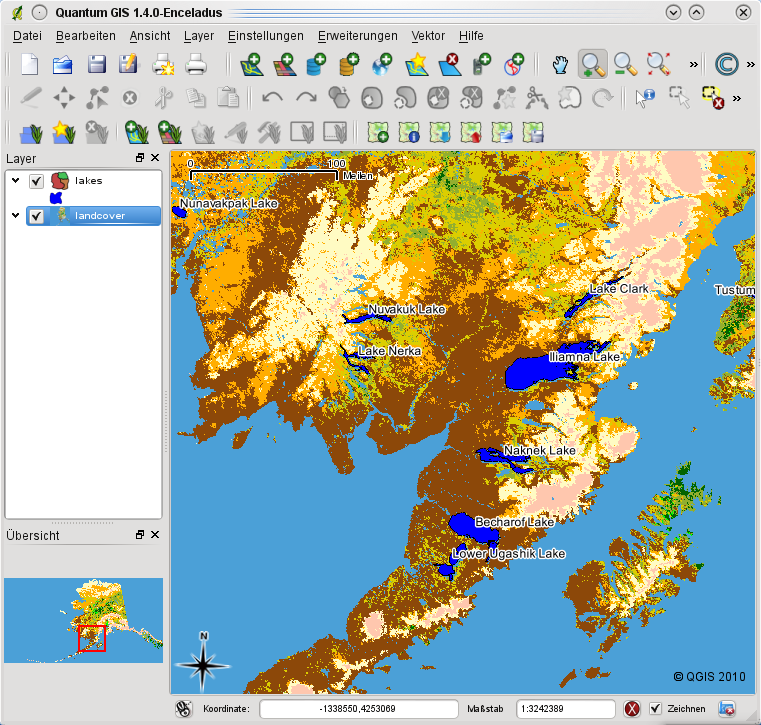
\includegraphics[clip=true, width=14cm]{simple_session}
\end{center}  
\end{figure}

You can see how easy it is to visualize raster and vector layers in 
QGIS. Let's move on to the sections that follow to learn more about the 
available functionality, features and settings and how to use them.
